\newcommand{\VS}{\vspace{6pt}}
\newcommand{\vt}[1]{\vec{#1}}

\chapter{Sampling} % Main chapter title

In this experiment we want to see if using a different subset of observations each iteration can reduce computational cost without negatively affecting performance.

\label{Chapter1} % For referencing the chapter elsewhere, use \ref{Chapter1} 

%----------------------------------------------------------------------------------------


\section{Description and reasoning}
\label{sec:ch5.sampling.desc}

Sampling is the process of selecting a representative part of a population. In machine learning sampling is done when creating a dataset, where each observation is a \emph{sample} of some unknown distribution. 

Sampling may also be done, a second time, when preparing the dataset. Clas\-si\-fi\-cation algorithms often require that all classes have a similar number of ob\-ser\-va\-tions, when this condition is not meet it is said that the dataset has \emph{sampling bias}. To avoid sampling bias, the dataset is resampled with another method called \emph{stratified random sampling}. This method consists on making a new dataset with only a subset of the observations, while imposing the restriction that all classes must have the same number of observations.

Because SVM computational cost is directly related to the amount of examples (i.e. samples), using only a subset of observations on each iteration can reduce this cost. In doing that, it is expected that performance will decrease, but we hope that in choosing a different subset each iteration, the performance will increase to levels similar to those we would see while using all data.

The reasoning for this last statement is that, although the algorithm only uses a subset of the data each iteration, by the time the algorithm finishes all data should've been used. Also, it is known that sampling improves generalization, thus we hope that this approx will reduce the gap between test and train error compared to the version with all data.

Further improvements may be introduced by reusing support vectors after the first iteration. Also, a dynamic sampling size may also be considered.

\section{Pseudocode formalization}

\textbf{Definitions:}

\begin{itemize}
    \item $X_0 = [\vt{x_0}, \vt{x_1}, \dotsc, \vt{x_k}]^T$ list of observations.
    \item $\vt{y} = [y_1, y_2, \dotsc, y_k]^T$ list of labels.
\end{itemize}

\begin{algorithm}[H]
    \DontPrintSemicolon
      \KwInput{$t, k$ \tcp*{$t$ = step, $k$ = number of samples, $0 < k \le |X_0|$}}
      \KwOutput{$\vt{r}$}
      \KwData{$X_0,\vt{y}$}
      $\vt{s} = [1,2, \dotsc, n]$ \tcp*{subset of surviving features}
      $\vt{r} = []$ \tcp*{feature ranked list}
      \While{$|\vt{s}| > 0$}
        {
            \tcc*[h]{Determine subset of examples by random sampling}\\
            $idx = \texttt{random\_sample}(|X_0|, k)$\VS

            \tcc*[h]{Restrict subset of examples to good feature indices}\\
            $X=X_0(idx,\vt{s})$\VS

            \tcc*[h]{Train the classifier}\\
            $\vt{\alpha} = \texttt{SVM-train(} X, y \texttt{)}$\VS

            \tcc*[h]{Compute the weight vector of dimension length $|\vt{s}|$}\\
            $\vt{w} = \sum_k{\vt{\alpha_k} \vt{y_k} \vt{x_k}}$\VS

            \tcc*[h]{Compute the ranking criteria}\\
            $\vt{c} = [(w_i)^2 \text{ for all $i$}]$\VS

            \tcc*[h]{Find the $t$ features with the smallest ranking criterion}\\
            $\vt{f} = \texttt{argsort}(\vt{c})(\ :t)$\VS

            \tcc*[h]{Update the feature ranking list}\\
            $\vt{r} = [\vt{s}(\vt{f}), ...\vt{r}]$\VS

            \tcc*[h]{Eliminate the features with the $t$ smallest ranking criterion}\\
            $\vt{s} = [[...\vt{s}(1:f_i - 1), ...\vt{s}(f_i + 1:|\vt{s}|)]$ for all $i]$
        }
    \caption{SVM-RFE with Random Sampling}
\end{algorithm}

\section{Results}

\begin{figure}[H]
    \centering
    \begin{subfigure}[b]{0.32\linewidth}
        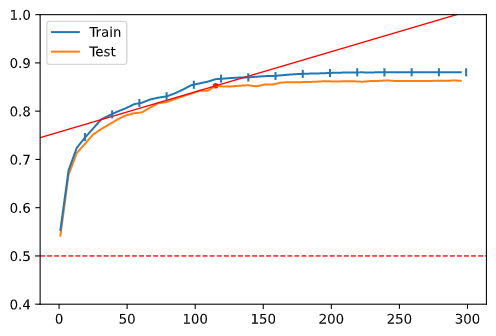
\includegraphics[width=\linewidth]{img/300-s20.png}
        \subcaption*{\textbf{A1.} $t = 20$}
    \end{subfigure}
    \begin{subfigure}[b]{0.32\linewidth}
        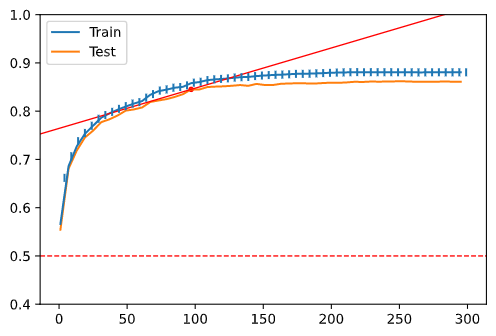
\includegraphics[width=\linewidth]{img/300-s5.png}
        \subcaption*{\textbf{A2.} $t = 5$}
    \end{subfigure}
    \begin{subfigure}[b]{0.32\linewidth}
        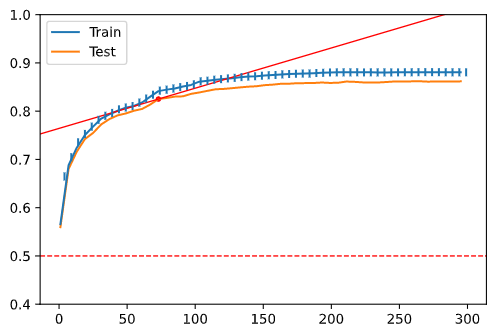
\includegraphics[width=\linewidth]{img/300-s5-05v.png}
        \subcaption*{\textbf{A3.} $t = 5$}
    \end{subfigure}
    \begin{subfigure}[b]{0.32\linewidth}
        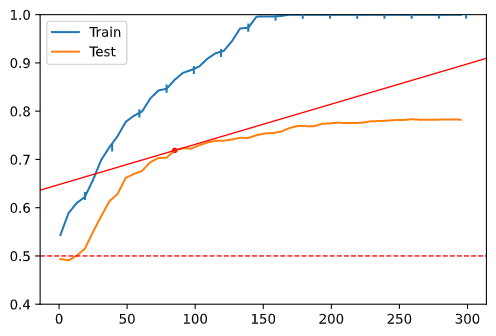
\includegraphics[width=\linewidth]{img/300-s20-p01-pre.png}
        \subcaption*{\textbf{B1.} $t = 20, k = 10\%$ PRE}
    \end{subfigure}
    \begin{subfigure}[b]{0.32\linewidth}
        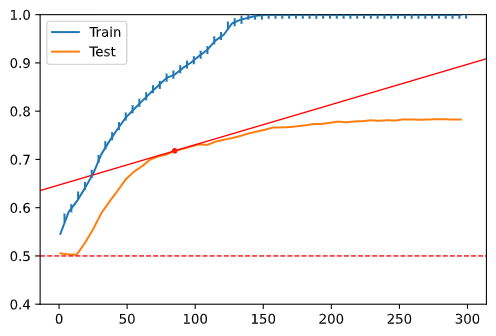
\includegraphics[width=\linewidth]{img/300-s5-p01-pre.png}
        \subcaption*{\textbf{B2.} $t = 5, k = 10\%$ PRE}
    \end{subfigure}
    \begin{subfigure}[b]{0.32\linewidth}
        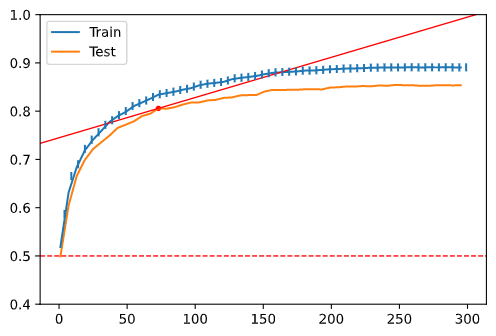
\includegraphics[width=\linewidth]{img/300-s5-p05-pre.png}
        \subcaption*{\textbf{B3.} $t = 5, k = 50\%$ PRE}
    \end{subfigure}
    \begin{subfigure}[b]{0.32\linewidth}
        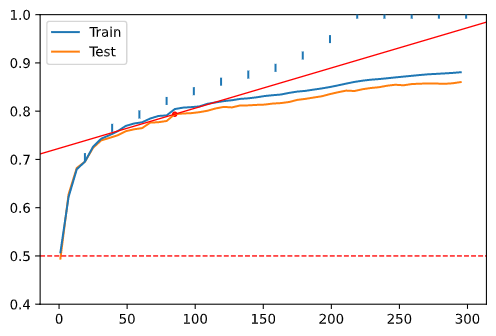
\includegraphics[width=\linewidth]{img/300-s20-p01.png}
        \subcaption*{\textbf{C1.} $t = 20, k = 10\%$}
    \end{subfigure}
    \begin{subfigure}[b]{0.32\linewidth}
        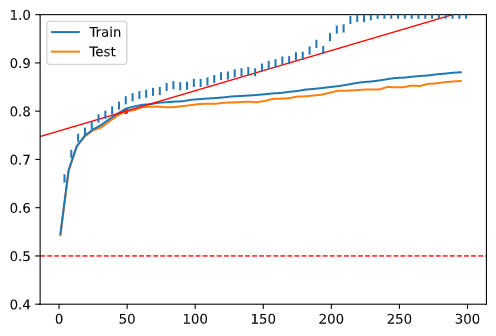
\includegraphics[width=\linewidth]{img/300-s5-p01.png}
        \subcaption*{\textbf{C2.} $t = 5, k = 10\%$}
    \end{subfigure}
    \begin{subfigure}[b]{0.32\linewidth}
        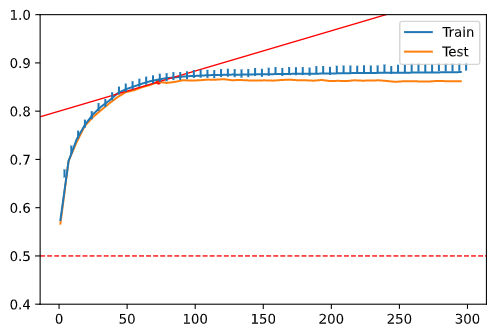
\includegraphics[width=\linewidth]{img/300-s5-p05.png}
        \subcaption*{\textbf{C3.} $t = 5, k = 50\%$}
    \end{subfigure}
    \caption{Grid comparing algorithms on each row \textbf{A-B-C} and the hyperparameter configuration for each \textbf{1} (step = 20), \textbf{2} (step = 5, sample = 10\%) and \textbf{3} (step = 5, sample = 50\%).}
    \label{fig:dynamicStep.vanilla.comp}
\end{figure}

\begin{table}[h]
    \centering
    \begin{tabular}{l | c c c|c c c|c c c}
        \toprule
        \multicolumn{1}{c}{} & \multicolumn{3}{c}{\textbf{1}} & \multicolumn{3}{c}{\textbf{2}} & \multicolumn{3}{c}{\textbf{3}}\\
        %\cline{2-4}\cline{5-7}\cline{8-10}
        \midrule
        &Feat.&Acc.&Score&Feat.&Acc.&Score&Feat.&Acc.&Score \\
        \midrule
        \textbf{A}&      115 & 85.25\% & 0.194 &      97 & 84.51\% & 0.189 &     73 & 82.51\% & 0.189\\
        \textbf{B}&      85 & 71.88\% & 0.281 &       85 & 71.79\% & 0.282 &     73 & 80.58\% & 0.204\\
        \textbf{C}&      85 & 79.38\% & 0.221 &       49 & 79.99\% & 0.193 &     73 & 86.08\% & 0.160\\
        \bottomrule
        \end{tabular}
    \caption{Perfomrance.}
\end{table}

\begin{table}[h]
    \centering
    \begin{tabular}{l | c c c | c c c | c c c }
        \toprule
        \multicolumn{1}{c}{} &\multicolumn{3}{c}{\textbf{1}} & \multicolumn{3}{c}{\textbf{2}} & \multicolumn{3}{c}{\textbf{3}}\\
        %\cline{2-4}\cline{5-7}\cline{8-10}
        \midrule
        &Iter.&Time ($s$) &Var. ($s^2$)&Iter.&Time ($s$) &Var. ($s^2$)&Iter.&Time ($s$) &Var. ($s^2$) \\
        \midrule
        \textbf{A}&      15 & 07.82 & 0.26 &      60 & 30.35 & 7.68 &     60 & 30.87 & 2.21\\
        \textbf{B}&      15 & 01.46 & 0.16 &      60 & 05.29 & 1.86 &     60 & 16.26 & 4.70\\
        \textbf{C}&      15 & 03.18 & 2.14 &      60 & 13.43 & 5.51 &     60 & 19.64 & 1.75\\
        \bottomrule
        \end{tabular}
    \caption{Times.}
\end{table}

Accuracy trade-off is 80\%. Problem is 8000 observations with 20-fold cross validation, 300 features, 100 informative.